\Needspace{10\baselineskip}
\section{数据、模型与工业闭环}
\label{sec:data}
本章说明数据采集、模型训练与量化、检查语义与前端形态。

\subsection{数据采集与审计}
数据集必须经板卡 \code{hdmi_in.readframe()} 采集，保证数据集像素与部署像素一致。
数据集实行清单化管理：来源、格式、训练/测试泄漏、空场景与实物分层审计，防泄漏审计含会话与实物双维划分及双哈希核对，共 13 组回归。
软件分层与一次检查的作业时序见图~\ref{fig:sw}。

\begin{figure}[H]\centering
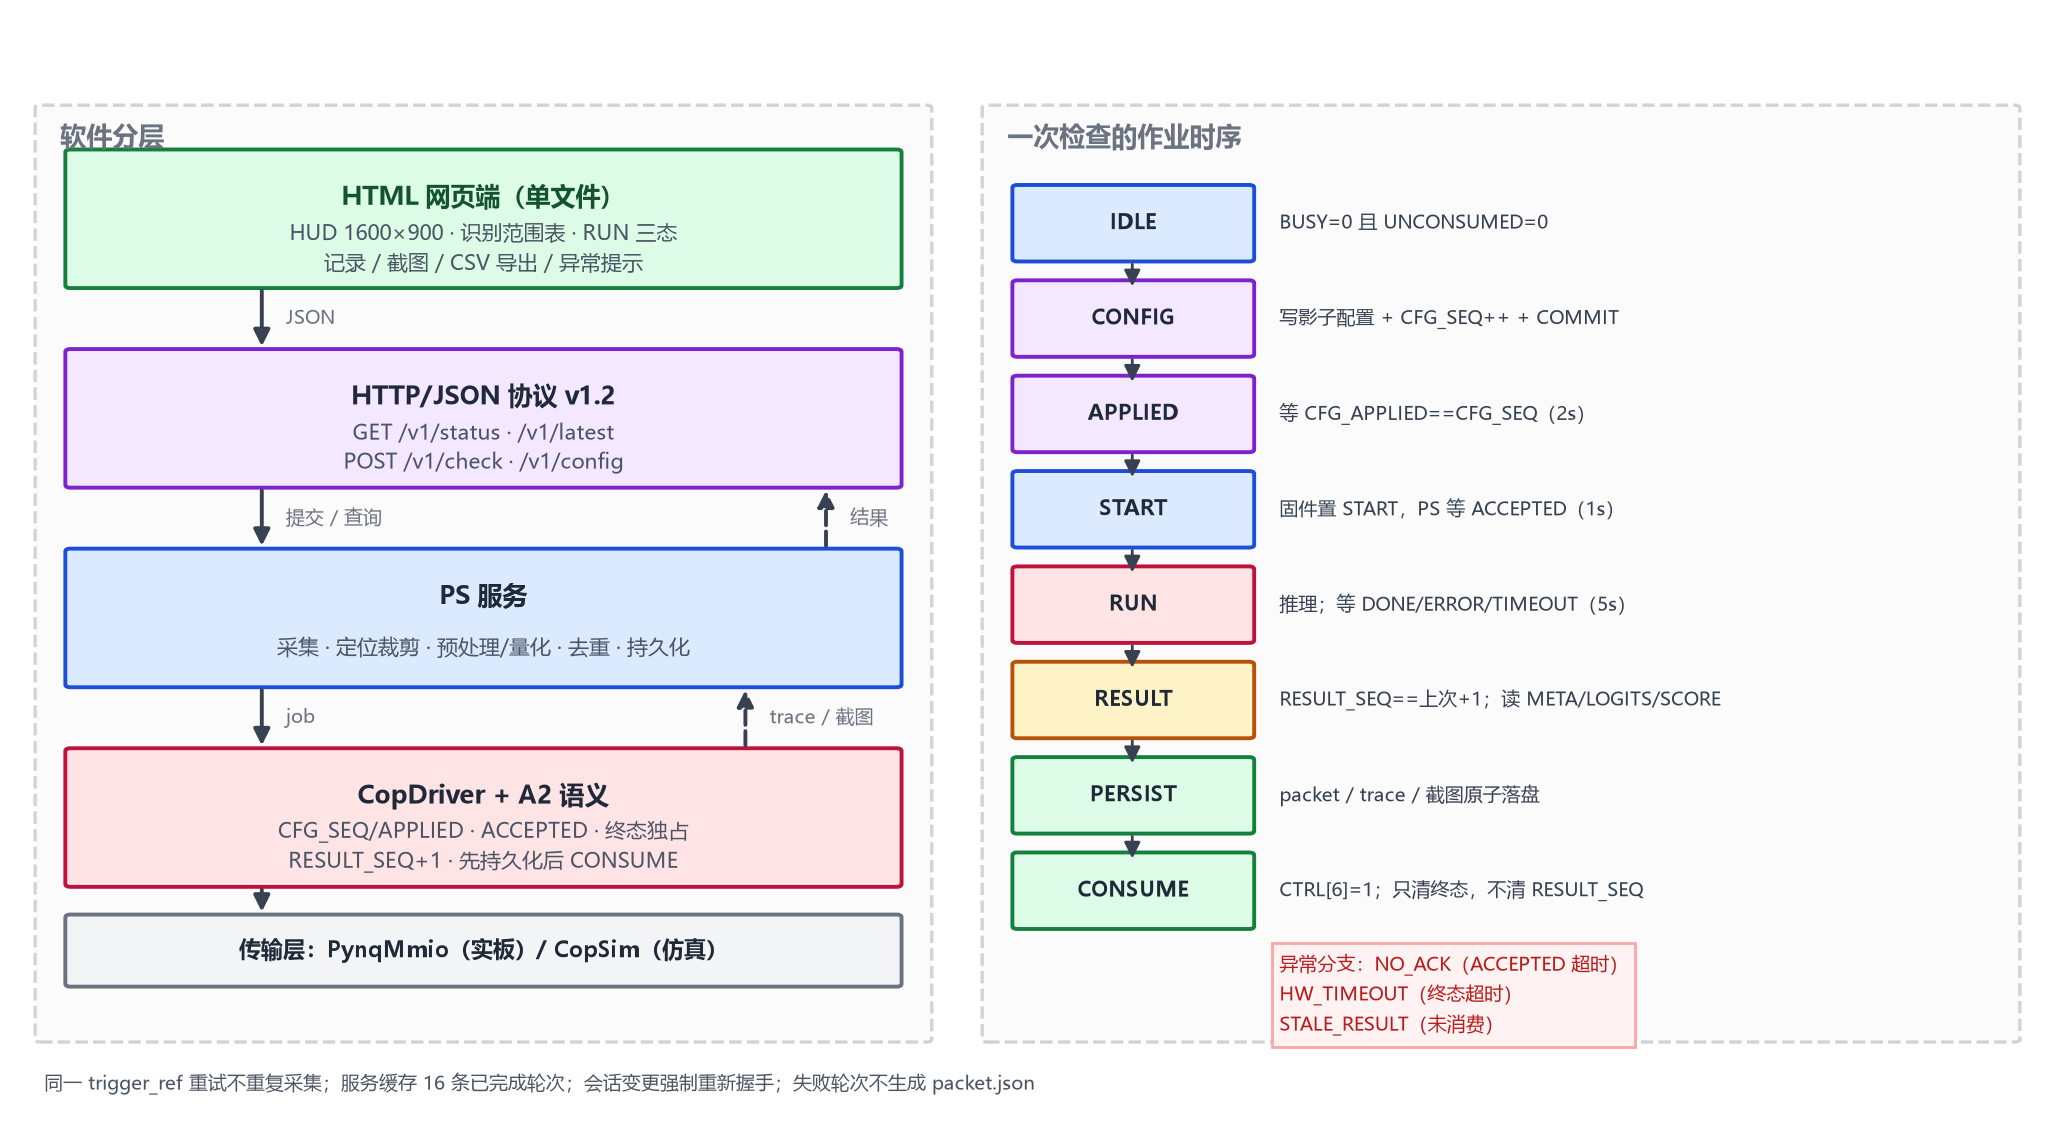
\includegraphics[width=0.98\linewidth]{fig_sw.png}
\caption{软件分层与一次检查的作业时序（仓库配图）}\label{fig:sw}
\end{figure}

\subsection{模型与量化}
分类网络为 64$\times$64 灰度小模型，按 C02 契约做训练后量化（PTQ）。
当前工作版本 r6：训练集 33 个 ROI，训练拟合与 PTQ 校准分类一致均为 33/33；未参与训练的清晰 5 螺母图 FP32 与 INT8 均为 5/5（含竖立螺母）。
权重、参数与复现命令见 CNN r6 证据包。

\subsection{留出对照与边界}
新摆放留出图（9 件，未参与训练与校准）对照结果见表~\ref{tab:holdout}。
全部 9 件被定位；FP32 与 INT8 各正确 8/9，均将 3 号垫圈判为螺母；分类一致性 9/9。
另有混合摆放 10 件图，定位与分类视觉复核 10/10，但未逐编号确认。
上述均为同工位开发对照，不是正式独立精度验收；换实物、换环境的泛化验收未实现，分类一致不能替代分类正确。

\begin{table}[H]\centering\small
\caption{CNN r6 留出摆放对照（9 件）}\label{tab:holdout}
\begin{tabularx}{\linewidth}{@{}P{42mm}P{30mm}Y@{}}\toprule
项目 & 结果 & 说明\\\midrule
定位 & 9/9 & 全部出框\\
FP32 分类正确 & 8/9 & 3 号垫圈判为螺母\\
INT8 分类正确 & 8/9 & 同上\\
分类一致性（FP32 vs INT8） & 9/9 & 不代表分类正确\\\bottomrule
\end{tabularx}\end{table}

\subsection{检查语义与记录}
检查按工单核对类别与数量，输出缺件、多余件、错料与复检提示。
重复帧不增加批次计数：记录资格绑定手动触发，属结构性保证。
异常事件附截图入档；记录导出为 UTF-8 BOM 的 CSV，避免 Excel 乱码。
断联、过期或无法确认的画面不显示为当前检查通过。

\subsection{前端形态}
前端为 HTML 网页端（\code{src/web_client}），经本机 Python 服务转发到板端，页面不直接访问硬件。
网页端已接入真实采集卡视频与板端轮次（2026-10-30 联调、2026-11-03 实验室复测）：
页面填写并下发工单（各类 0--10 件、合计 1--10 件），板端校验回显后配置号递增，未应用时禁止开始检查；
结果按接收时刻计龄 4.5\,s，超龄、断联或配置不符立即撤框；自动轮询默认暂停、单请求在途；
手动有效轮次按会话与检查编号去重，记录导出为 UTF-8 BOM 的 CSV。
当前按单页使用：同会话的第二个客户端会争用配置并导致连接中断，属已知限制。
桌面程序已于 2026-10-28 全套退役，历史记录保留在 git 历史与当日协作日志中。
\FloatBarrier
